\documentclass[a4paper,12pt]{scrartcl}
\usepackage[utf8]{inputenc}
\usepackage[UKenglish]{isodate}
\usepackage{csquotes}
\usepackage{graphicx}
\usepackage{wrapfig}
\usepackage{enumitem}
\usepackage{pdflscape}
\usepackage[toc,page]{appendix}
\usepackage{geometry}
\usepackage{hyperref}
\usepackage{cleveref}
\usepackage{listings}
\usepackage{csvsimple}
\usepackage{booktabs}
\usepackage{longtable}
\usepackage{caption}
\usepackage{subcaption}
\usepackage[colorinlistoftodos]{todonotes}
\usepackage[british]{babel}
\usepackage{float}
%\usepackage[margin=1in]{geometry}
\usepackage{listings}
\usepackage{color}
 
\definecolor{codegreen}{rgb}{0,0.6,0}
\definecolor{codegray}{rgb}{0.5,0.5,0.5}
\definecolor{codepurple}{rgb}{0.58,0,0.82}
\definecolor{backcolour}{rgb}{0.95,0.95,0.92}
 
\lstdefinestyle{mystyle}{
	language=PHP,
    backgroundcolor=\color{backcolour},   
    commentstyle=\color{codegray},
    keywordstyle=\color{magenta},
    numberstyle=\tiny\color{codegray},
    stringstyle=\color{codegreen},
    basicstyle=\footnotesize,
    breakatwhitespace=false,         
    breaklines=true,                 
    captionpos=b,                    
    keepspaces=true,                 
    numbers=left,                    
    numbersep=5pt,                  
    showspaces=false,                
    showstringspaces=false,
    showtabs=false,                  
    tabsize=3,
    morekeywords={ new, __halt_compiler, abstract, and, array, as, break, callable, case, catch, class, clone, const, continue, declare, default, die, do, echo, else, elseif, empty, enddeclare, endfor, endforeach, endif, endswitch, endwhile, eval, exit, extends, final, for, foreach, function, global, goto, if, implements, include, include_once, instanceof, insteadof, interface, isset, list, namespace, new, or, print, private, protected, public, require, require_once, return, static, switch, throw, trait, try, unset, use, var, while, xor}
}

\lstset{language=Java,
  showspaces=false,
  showtabs=false,
  breaklines=true,
  showstringspaces=false,
  breakatwhitespace=true,
  commentstyle=\color{pgreen},
  keywordstyle=\color{pblue},
  stringstyle=\color{pred},
  basicstyle=\ttfamily,
  moredelim=[il][\textcolor{pgrey}]{$$},
  moredelim=[is][\textcolor{pgrey}]{\%\%}{\%\%}
}
 
\lstset{style=mystyle}

\graphicspath{ {images/} }
\usepackage[
	backend=biber,
	style=ieee,
	]{biblatex}

\addbibresource{references.bib}

\title{829H1 Real-Time Embedded Systems Final Report}
\author{Candidate No: 105936}
\date{\today}

\begin{document}
	
	\begin{titlepage}
		\maketitle
	\end{titlepage}
	
	\tableofcontents
	\newpage

	\section{Abstract}
	{
		The IoT space is full of applications and devices to make life easier this project has also been inspired by this trend. The main section of this report is focused on how to connect the freedom K64F\cite{nxpproducts2014} to an external API and display text on the application shield. It looks into the process of displaying current weather information on the application shields display. Please note a digital copy of this document can be found at  \url{https://github.com/jamesfernando94/UniversityDocuments/raw/master/4-RealTimeEmbeddedSystems/FinalReport/RealTimeEmbeddedSystemsFinalReport.pdf} it is advised to use this due to the number of links in the document.
	}

	\section{Introduction}
	{
		This report focuses on using the FRDM-K64F\cite{nxpproducts2014} as a connected device to display weather information on the application shields display. Developing for real time systems relies on ensuring that there is no delay for the program in terms of using interrupts correctly and ensuring the program runs quickly. I will start by going through the exercises I completed during the lab sessions before going on to how I created the weather application which runs on the board. 
	}
	
	\section{Exercises}
	{
		I conducted a number of exercises/experiments over the course of the term and learnt a number of ways in which the outputs of the board can be used and other programming constructs. In this section I will go over what was learnt and how it helped to complete the project.
		\subsection{Parallel IO}
		{
			This was a relatively gentle introduction on programming for embedded systems. It allowed me to get used to how to use the mbed IDE and how developing for the board works. This exercise was based on direct programming where the binaries are complied to run on the specific hardware. This is sightly different from my background in programming for computers where a program is complied for an Operating system or some other intermediate interface between the program and the hardware. 
		}
		\subsection{Interrupt and Timers}
		{
			Although I did not use the timer functionality in the end for my project, I found the interrupts to be very useful and vital for real time embedded systems as it is necessary for systems to be able to manage changes and be able to react to important information. I ended up using the interrupts feature to deal with the inputs from the joystick although I had to go further and use mbed events\cite{Jongboom2018} as well so that I was able to output to the various displays. This is because it is not possible to output to a serial communication from an interrupt.
			\begin{table}[]
				\centering
				\begin{tabular}{|c|c|c|c|}
					\hline
					\textbf{\begin{tabular}[c]{@{}c@{}}Character\\ Length\end{tabular}} & \textbf{String} & \textbf{\begin{tabular}[c]{@{}c@{}}Time taken to\\ print to screen\end{tabular}} & \textbf{\begin{tabular}[c]{@{}c@{}}Difference to one\\ fewer character length\end{tabular}} \\ \hline
					0 &  & 0.000019 &  \\ \hline
					1 & a & 0.002075 & 0.002056 \\ \hline
					2 & aa & 0.003114 & 0.001039 \\ \hline
					3 & aaa & 0.004154 & 0.00104 \\ \hline
					4 & aaaa & 0.005194 & 0.00104 \\ \hline
					5 & aaaaa & 0.006235 & 0.001041 \\ \hline
					6 & aaaaaa & 0.007275 & 0.00104 \\ \hline
					7 & aaaaaaa & 0.008314 & 0.001039 \\ \hline
					8 & aaaaaaaa & 0.009355 & 0.001041 \\ \hline
					9 & aaaaaaaaa & 0.010395 & 0.00104 \\ \hline
					10 & aaaaaaaaaa & 0.011435 & 0.00104 \\ \hline
				\end{tabular}
				\caption{Showing the time taken to print a string to the screen compared to the character length.}
				\label{tbl:TimeToPrintToScreen}
			\end{table} 
			\Cref{tbl:TimeToPrintToScreen} is an example of some fo the results I found while working on the experiments in this section. This experiment was using timers to measure how long it took to write a string to the screen depending on its length. The code for this experiment can be found in \cref{appendix:write-string-timer}.
		}
		\subsection{Power Width Modulation}
		{
			This exercise was not particularly useful when building my project however it does provide a good introduction on how motor and other devices work these provide a useful introduction on how to use the oscilloscope and work that would be completed in the next section.
		}
		\subsection{Serial Communications}
		{
			This helped cement knowledge about how serial communications work while also providing a bit of background information on parallel communication. This was one of the more complicated exercises although it did allow for the learning of a number of parts of serial communications, such as the purpose of different lines. For example the clock line, MISO, MOSI. I was also able to learn about the different clock modes which would change when the data bits were sent compared to the clock line values. Although the USB mouse functionality was relatively interesting and provided a small insight on the number of features which are available on the board.
			\begin{figure}[h]
				\centering
				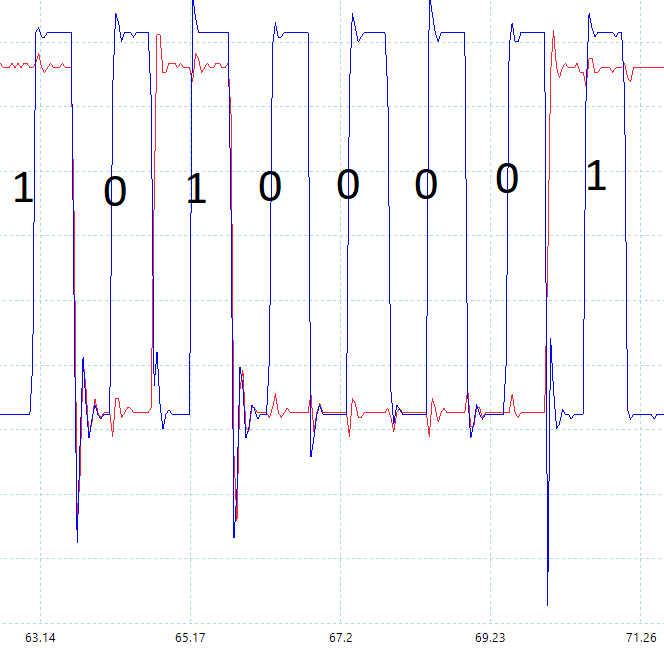
\includegraphics[width=0.5\textwidth]{Task1-Edited}
				\caption{An Image showing the output on the oscilloscope when outputting the byte 10100001}
				\label{img:AnotatedByteOutput}
			\end{figure}
			\Cref{img:AnotatedByteOutput} shows how each signal is interpreted when the byte is transmitted.
		}
		\subsection{Ethernet Connections}
		{
			This exercise taught me the basics about network communications and provided some of the basic ideas for what I could produce for my project. The IBM application clearly showed what sensors were available to be used.
		}
	}

	\section{Project}
	{
		The main plan for the project was to create a program which would make the device a simple to use weather station of sorts. It would get its current location via it's IP address and then query a external API for the current weather conditions before displaying the information on the screen. The code for the application can be found at \cref{appendix:Weather-app-project} and the full repository can be accessed at \url{https://os.mbed.com/users/jamesfernando/code/frdm_project/}.
		\subsection{Getting the current public IP Address}
		{
			The first part of the program was to get the board to get it's own ip address allowing the board to query the location for the correct IP. To do this I needed to get the current public IP address of the board using the code \lstinline|EthernetInterface.getIPAddress()| unfortunately this only returned the internal IP address. Therefore, I had to use a public API to get the IP address for this I used \url{https://api.ipify.org}\cite{Degges}. This would send off a http request to the address and then read the received text back. To send the http request I had to use the \url{https://os.mbed.com/teams/sandbox/code/mbed-http/} library simply importing this library didn't work therefore I had to fork the http examples repository found at \url{https://os.mbed.com/teams/sandbox/code/http-example/} and modify it for my purposes. The code I used for this task can be found at \cref{appendix:get-IP-Address-Via-HTTP}.
		}
		\subsection{Displaying on the LCD}
		{
			This was fairly simple to implement compared to the http library. As all I needed to do was import the library from \url{https://os.mbed.com/users/chris/code/C12832/} and use the example from \url{https://os.mbed.com/users/chris/code/app-shield-LCD/file/f8ef5e45e488/main.cpp/} as guidance on how to use the library. The code I used for this can be found at \cref{appendix:display-to-LCD}.
		}
		\subsection{Re-factoring the code}
		{
			After implementing the function to get the IP address and display it to the screen I realised that if I wanted to display each of the individual pieces of information I would have to change the layout of the code to make this easier. This meant that I would need to create a number of functions to manage what would be displayed and how to change the information on the display.
		}
		\subsection{Using the joystick to scroll through the display}
		{
			To make use of the joystick I only had to add \lstinline|InterruptIn joy_up(A2);| for up and down and then make use of the inputs for this. My initial plan was to use the interrupt to update the screens display however it is not possible to call serial communications from an interrupt meaning I cannot use the printf to the LCD or to the debug USB. To overcome this issue I need to use mbed events to do this I used information from the blog \url{https://os.mbed.com/blog/entry/Simplify-your-code-with-mbed-events/}\cite{Jongboom2018}. This would allow me to add functions to be called on a separate thread. After this I now had the basic layout of the system working so all I needed to do was to add functionality to get the location and then weather information. The code I used for this can be found at \cref{appendix:use-joystick}.
		}
		\subsection{Getting the Location}
		{
			Obtaining the location was simple as all I had to do was use the code from earlier to get the IP address, but change the URL to an API which would get the location. I also needed to parse the result to make use of the individual JSON values(I.E. the Latitude and Longitude values). To do this I used this library \url{https://os.mbed.com/users/samux/code/MbedJSONValue/} as it had some documentation on how to use it. This allowed me to relatively easily obtain the latitude and longitude as strings. The code I used for this can be found at \cref{appendix:get-location}.
		}
		\subsection{Displaying the Weather Information}
		{
			After I had the obtained the coordinates All I needed to do was to use the API from \url{https://openweathermap.org/api} to get the weather information for the coordinates I obtained earlier. As I was able to display the temperature fairly quickly I decided on adding a description of the weather to the display. The  only slightly complicated thing was converting the temperature value from a double to a string to help me with this I searched stack overflow and found this result \url{https://stackoverflow.com/a/332132}\cite{Schaub2008}. The code I used for this can be found at \cref{appendix:get-weather-info}.
		}
	}
	
	\section{Analysis}
	{
		\subsection{Program Information/User Guide}
		{
			The idea of this program is that all you have to do is plug it in and it works the rest out for you. Therefore to get it working all you need to do is connect the USB and Ethernet and then wait for it to load information. You are able to scroll through the information using the joystick before it loads but all it will read is \lstinline|waiting...| but it will refresh once the data is obtained.
		}
		\subsection{Review}\label{sec:Review}
		{
			I've used the device a couple of times since creating it and it is relatively useful as it is quick to boot up and simply displays the temperature to an accurate level. There are a few improvements which can be made such as remembering the last option selected therefore when the device is connected it does not default to the ip address display. Another would be that it takes quite a long time to get the IP address. I'm not sure if that is because it is the first http call therefore there is some setup which must be done or the API is a bit slow but it would probably be worth looking into using other API's to get the IP address to see if they are quicker. Another improvement would be to make the values update every so often or add the functionality so that clicking centre on the joystick would update the values as the only way to do it currently is to reboot the device. One final improvement which could be made is the device could display an icon depending on the weather conditions. 
		}
	}
	
	\section{Conclusion}
	{
		Over the course of the module I've learnt a fair amount about developing for embedded systems although I feel that there is much more which can be learnt. I feel that the  project I've created is of usable quality, although there are some improvements which can be made and have been mentioned in \cref{sec:Review}. I feel I completed the project I set out to create therefore this has been a success.
	}
	
	\newpage
	\begin{appendices}
	\label{Appendix:start}
	\section{Lab Exercise 1}
	{
		\subsection{Part 1}
		{
			\label{appendix:ex1-1}
			\lstinputlisting[language=c++]{CodeListings/Ex1/mainPart1.cpp}
		}
		\subsection{Part 2}
		{
			\label{appendix:ex1-2}
			\lstinputlisting[language=c++]{CodeListings/Ex1/mainPart2.cpp}
		}
		\subsection{Part 3}
		{
			\label{appendix:ex1-3}
			\lstinputlisting[language=c++]{CodeListings/Ex1/mainPart3.cpp}
		}
	}
	\section{Lab Exercise 2}
	{
		\label{appendix:ex2}
		\subsection{Part 1 - Master Program}
		{
			\label{appendix:ex2-1}
			\lstinputlisting[language=c++]{CodeListings/Ex2/main-master.cpp}
		}
		\subsection{Part 2 - Slave Program}
		{
			\label{appendix:ex2-2}
			\lstinputlisting[language=c++]{CodeListings/Ex2/main-slave.cpp}
		}
	}

\end{appendices}
	\printbibliography[heading=bibintoc,title=References]
\end{document}
